%%%%%%%%%%%%%%%%%%%%%%%%%%%%%%%%%%%%%%%%%%%%%%%%%%%%%%%%%%%%%%%%%%%%%%%%%%%%%%%
% CASE STUDY TEMPLATE - Programming and Problem Solving
% Author: Brendan Shea, PhD
% Course: Programming and Problem Solving
% Rochester Community and Technical College
%%%%%%%%%%%%%%%%%%%%%%%%%%%%%%%%%%%%%%%%%%%%%%%%%%%%%%%%%%%%%%%%%%%%%%%%%%%%%%%

\documentclass[11pt,letterpaper]{article}

%---------- PACKAGES ----------%
\usepackage[margin=1in, headheight=22pt]{geometry}
\usepackage[T1]{fontenc}
\usepackage{xcolor}
\usepackage{tcolorbox}
\usepackage{graphicx}
\usepackage{titlesec}
\usepackage{enumitem}
\usepackage{fancyhdr}
\usepackage{listings}
\usepackage{hyperref}
\usepackage{multicol}
\usepackage{booktabs}
\usepackage{tikz}
\usepackage{float}
\usepackage{amssymb}
\usepackage{amsmath}
\usepackage{pifont}

% TikZ libraries
\usetikzlibrary{shapes.geometric, arrows.meta, positioning, calc, backgrounds, fit, matrix, decorations.pathreplacing}

% Load tcolorbox libraries
\tcbuselibrary{skins,breakable,listings,listingsutf8}

%---------- COLOR DEFINITIONS ----------%
\definecolor{csprimary}{HTML}{2C3E50}
\definecolor{cssecondary}{HTML}{E74C3C}
\definecolor{cstertiary}{HTML}{3498DB}
\definecolor{csaccent}{HTML}{27AE60}
\definecolor{cswarm}{HTML}{F39C12}
\definecolor{cslight}{HTML}{ECF0F1}
\definecolor{csdark}{HTML}{1A252F}

% Syntax highlighting colors
\definecolor{codegreen}{HTML}{27AE60}
\definecolor{codepurple}{HTML}{9B59B6}
\definecolor{codeorange}{HTML}{E67E22}
\definecolor{codeblue}{HTML}{3498DB}
\definecolor{codegray}{HTML}{95A5A6}
\definecolor{codestring}{HTML}{E74C3C}
\definecolor{codebg}{HTML}{1E2A38}

%---------- CASE STUDY METADATA ----------%
\newcommand{\cstitle}{Searching the Entire Internet}
\newcommand{\cssubtitle}{How Google Finds Answers in Half a Second}
\newcommand{\csauthor}{Brendan Shea, PhD}
\newcommand{\cscourse}{Programming and Problem Solving}
\newcommand{\csinstitution}{Rochester Community and Technical College}
\newcommand{\csdate}{\today}

%---------- LISTINGS CONFIGURATION ----------%
\lstdefinestyle{basestyle}{
    backgroundcolor=\color{codebg},
    basicstyle=\ttfamily\small\color{white},
    breakatwhitespace=false,
    breaklines=true,
    captionpos=b,
    keepspaces=true,
    showspaces=false,
    showstringspaces=false,
    showtabs=false,
    tabsize=4,
    frame=none,
    xleftmargin=4mm,
    xrightmargin=4mm,
    aboveskip=0pt,
    belowskip=0pt,
}

\lstdefinestyle{javastyle}{
    style=basestyle,
    language=Java,
    keywordstyle=\color{codeblue}\bfseries,
    commentstyle=\color{codegray}\itshape,
    stringstyle=\color{codestring},
    morekeywords={String, Scanner, System, var, boolean, Math, List, Map, HashMap, ArrayList, Set, HashSet},
}

%---------- CUSTOM ENVIRONMENTS ----------%
\newcommand{\keyterm}[1]{\textbf{\textcolor{cssecondary}{#1}}}

\newtcolorbox{conceptbox}[1][]{
    enhanced,
    colback=cslight,
    colframe=csprimary,
    fonttitle=\bfseries\color{white},
    title=#1,
    attach boxed title to top left={yshift=-2mm, xshift=5mm},
    boxed title style={colback=csprimary},
    breakable
}

\newtcolorbox{historybox}[1][]{
    enhanced,
    colback=codepurple!8,
    colframe=codepurple,
    fonttitle=\bfseries\color{white},
    title=#1,
    attach boxed title to top left={yshift=-2mm, xshift=5mm},
    boxed title style={colback=codepurple},
    breakable
}

\newtcolorbox{mathbox}[1][]{
    enhanced,
    colback=cstertiary!8,
    colframe=cstertiary,
    fonttitle=\bfseries\color{white},
    title=#1,
    attach boxed title to top left={yshift=-2mm, xshift=5mm},
    boxed title style={colback=cstertiary},
    breakable
}

\newtcblisting{javacode}[1][]{
    enhanced,
    colback=codebg,
    colframe=csaccent,
    colupper=white,
    fonttitle=\bfseries\color{white},
    title=#1,
    attach boxed title to top left={yshift=-2mm, xshift=5mm},
    boxed title style={colback=csaccent},
    left=0mm, right=0mm, top=2mm, bottom=2mm,
    boxrule=1pt,
    breakable,
    pad at break=2mm,
    listing only,
    listing options={style=javastyle}
}

\newtcolorbox{questionbox}{
    enhanced,
    colback=cswarm!10,
    colframe=cswarm,
    fonttitle=\bfseries\color{white},
    title=Discussion Questions,
    attach boxed title to top center={yshift=-2mm},
    boxed title style={colback=cswarm},
    breakable
}

\newtcolorbox{glossarybox}{
    enhanced,
    colback=cslight,
    colframe=csprimary,
    fonttitle=\bfseries\color{white},
    title=Glossary of Key Terms,
    attach boxed title to top center={yshift=-2mm},
    boxed title style={colback=csprimary},
    breakable
}

%---------- HEADER/FOOTER ----------%
\pagestyle{fancy}
\fancyhf{}
\fancyhead[L]{\small\textcolor{csprimary}{\cscourse}}
\fancyhead[R]{\small\textcolor{csprimary}{Case Study}}
\fancyfoot[C]{\thepage}
\renewcommand{\headrulewidth}{0.4pt}
\renewcommand{\headrule}{\hbox to\headwidth{\color{csprimary}\leaders\hrule height \headrulewidth\hfill}}

%---------- SECTION FORMATTING ----------%
\titleformat{\section}
    {\Large\bfseries\color{csprimary}}
    {\thesection}{1em}{}[\color{cssecondary}\titlerule]
    
\titleformat{\subsection}
    {\large\bfseries\color{cstertiary}}
    {\thesubsection}{1em}{}

%---------- HYPERLINK SETTINGS ----------%
\hypersetup{
    colorlinks=true,
    linkcolor=cstertiary,
    urlcolor=cstertiary
}

%%%%%%%%%%%%%%%%%%%%%%%%%%%%%%%%%%%%%%%%%%%%%%%%%%%%%%%%%%%%%%%%%%%%%%%%%%%%%%%
\begin{document}

%---------- TITLE BLOCK ----------%
\begin{tcolorbox}[
    enhanced,
    colback=csprimary,
    colframe=csprimary,
    arc=0mm,
    left=10mm, right=10mm, top=8mm, bottom=8mm
]
\begin{center}
    {\huge\bfseries\color{white}\cstitle}\\[3mm]
    {\Large\color{cslight}\cssubtitle}\\[5mm]
    \textcolor{cssecondary}{\rule{0.5\textwidth}{1pt}}\\[5mm]
    {\large\color{white}\csauthor}\\[2mm]
    {\normalsize\color{cslight}\cscourse\ $\bullet$ \csinstitution}
\end{center}
\end{tcolorbox}

\vspace{5mm}

%---------- INTRODUCTION ----------%
\section*{Introduction}

Type a question into Google. In roughly half a second, you receive results drawn from hundreds of billions of web pages. The scale is staggering: if you could check one web page per second, it would take you over 15,000 years to examine what Google searches in 0.5 seconds.

How is this possible? The answer involves clever data structures, distributed computing across millions of servers, and an algorithm invented by two Stanford graduate students that revolutionized how we think about information. Understanding web search illuminates fundamental concepts in computer science: indexing, graph algorithms, parallel processing, and the trade-offs between storage and computation.

This case study traces the journey of a search query---from the moment you press Enter to the instant results appear. Along the way, we'll explore the history of search engines, peek inside Google's architecture, and examine how artificial intelligence is transforming search in the 2020s.

\begin{conceptbox}[The Scale of the Problem]
\begin{itemize}[leftmargin=*, itemsep=2pt]
    \item The indexed web contains over \textbf{400 billion pages}
    \item Google processes over \textbf{8.5 billion searches per day}
    \item Average response time: \textbf{less than 0.5 seconds}
    \item Google operates \textbf{millions of servers} across 40+ data centers worldwide
\end{itemize}
The fundamental insight: you don't actually search the web---you search \textit{Google's index} of the web.
\end{conceptbox}

%---------- BEFORE GOOGLE ----------%
\section{Before Google: The Search Problem}

\begin{historybox}[The Early Days of Web Search]
The first web search tool, ``Wandex,'' appeared in 1993, created by Matthew Gray at MIT. Early search engines like AltaVista (1995), Lycos (1994), and Yahoo! (originally a hand-curated directory) helped users navigate the growing web. But they shared a fundamental problem: as the web exploded in size, search quality collapsed.

These engines primarily matched keywords---if your page contained the words a user searched for, it appeared in results. Website owners quickly learned to stuff invisible keywords into their pages (``keyword stuffing''), and search results became polluted with spam and irrelevant content. By the late 1990s, finding useful information felt like searching for a needle in an exponentially growing haystack.
\end{historybox}

The challenge wasn't just finding pages that \textit{contained} your search terms---it was finding pages that were actually \textit{useful}. A search for ``computer science'' might match millions of pages, but which ones deserve to appear first? Keyword frequency alone couldn't answer this question.

%---------- CRAWLING ----------%
\section{Step 1: Crawling the Web}

Before Google can search anything, it must first discover what exists. This is the job of the \keyterm{web crawler} (also called a ``spider'' or ``bot'')---a program that systematically browses the web, following links from page to page.

\begin{center}
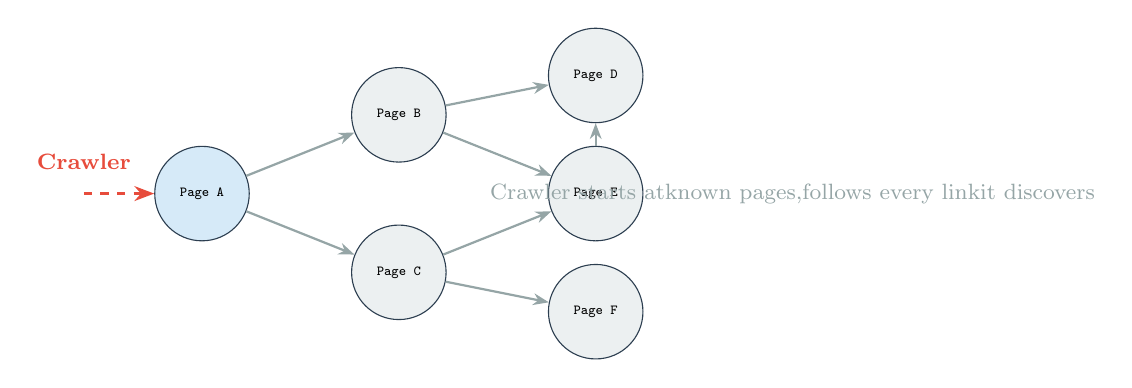
\begin{tikzpicture}[
    page/.style={circle, draw=csprimary, fill=#1, minimum size=12mm, font=\tiny\ttfamily},
    arrow/.style={-{Stealth[length=2mm]}, thick, color=codegray},
    crawl/.style={-{Stealth[length=2.5mm]}, very thick, color=cssecondary}
]

% Web pages as nodes
\node[page=cstertiary!20] (a) at (0,0) {Page A};
\node[page=cslight] (b) at (2.5,1) {Page B};
\node[page=cslight] (c) at (2.5,-1) {Page C};
\node[page=cslight] (d) at (5,1.5) {Page D};
\node[page=cslight] (e) at (5,0) {Page E};
\node[page=cslight] (f) at (5,-1.5) {Page F};

% Links between pages
\draw[arrow] (a) -- (b);
\draw[arrow] (a) -- (c);
\draw[arrow] (b) -- (d);
\draw[arrow] (b) -- (e);
\draw[arrow] (c) -- (e);
\draw[arrow] (c) -- (f);
\draw[arrow] (e) -- (d);

% Crawler path
\draw[crawl, dashed] (-1.5,0) -- (a);
\node[font=\footnotesize\bfseries, color=cssecondary] at (-1.5,0.4) {Crawler};

% Legend
\node[font=\footnotesize, color=codegray, align=left] at (7.5,0) {Crawler starts at\newline known pages,\newline follows every link\newline it discovers};

\end{tikzpicture}
\end{center}

The crawler works like this:
\begin{enumerate}[itemsep=2pt]
    \item Start with a list of known URLs (seed pages)
    \item Download a page and extract all links from it
    \item Add new links to the queue of pages to visit
    \item Record the page's content for indexing
    \item Repeat---forever
\end{enumerate}

Google's crawler, called \keyterm{Googlebot}, continuously crawls the web, revisiting pages to detect changes. Popular sites might be recrawled every few minutes; obscure pages might wait weeks between visits. The crawler must also respect \texttt{robots.txt} files, which tell crawlers which parts of a site they're allowed to access.

\begin{javacode}[Simplified Crawler Logic]
public void crawl(String startUrl) {
    Queue<String> toVisit = new LinkedList<>();
    Set<String> visited = new HashSet<>();
    
    toVisit.add(startUrl);
    
    while (!toVisit.isEmpty()) {
        String url = toVisit.poll();
        
        if (visited.contains(url)) continue;  // Skip if already seen
        visited.add(url);
        
        String pageContent = downloadPage(url);
        saveForIndexing(url, pageContent);
        
        // Find all links on this page and add them to queue
        List<String> links = extractLinks(pageContent);
        for (String link : links) {
            if (!visited.contains(link)) {
                toVisit.add(link);
            }
        }
    }
}
\end{javacode}

The real Googlebot is vastly more sophisticated---handling authentication, JavaScript rendering, politeness delays (not overwhelming servers with requests), and prioritizing which pages to crawl first---but this captures the core idea.

%---------- INDEXING ----------%
\section{Step 2: Building the Index}

Crawling gives us billions of pages. But we can't search through raw pages quickly enough---imagine reading every book in every library to find one fact. Instead, we build an \keyterm{index}: a data structure optimized for fast lookups.

Think about the index at the back of a textbook. Instead of reading every page to find where ``algorithm'' is mentioned, you look up ``algorithm'' in the index and get a list of page numbers. Web search works the same way, using a structure called an \keyterm{inverted index}.

\begin{center}
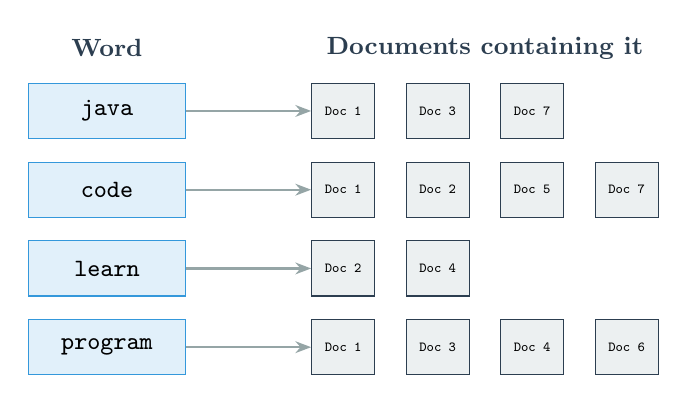
\begin{tikzpicture}[
    word/.style={rectangle, draw=cstertiary, fill=cstertiary!15, minimum width=20mm, minimum height=7mm, font=\small\ttfamily},
    doc/.style={rectangle, draw=csprimary, fill=cslight, minimum width=8mm, minimum height=7mm, font=\tiny\ttfamily},
    arrow/.style={-{Stealth[length=2mm]}, thick, color=codegray}
]

% Words
\node[word] (w1) at (0,1.5) {java};
\node[word] (w2) at (0,0.5) {code};
\node[word] (w3) at (0,-0.5) {learn};
\node[word] (w4) at (0,-1.5) {program};

% Document lists
\node[doc] (d1a) at (3,1.5) {Doc 1};
\node[doc] (d1b) at (4.2,1.5) {Doc 3};
\node[doc] (d1c) at (5.4,1.5) {Doc 7};

\node[doc] (d2a) at (3,0.5) {Doc 1};
\node[doc] (d2b) at (4.2,0.5) {Doc 2};
\node[doc] (d2c) at (5.4,0.5) {Doc 5};
\node[doc] (d2d) at (6.6,0.5) {Doc 7};

\node[doc] (d3a) at (3,-0.5) {Doc 2};
\node[doc] (d3b) at (4.2,-0.5) {Doc 4};

\node[doc] (d4a) at (3,-1.5) {Doc 1};
\node[doc] (d4b) at (4.2,-1.5) {Doc 3};
\node[doc] (d4c) at (5.4,-1.5) {Doc 4};
\node[doc] (d4d) at (6.6,-1.5) {Doc 6};

% Arrows
\draw[arrow] (w1) -- (d1a);
\draw[arrow] (w2) -- (d2a);
\draw[arrow] (w3) -- (d3a);
\draw[arrow] (w4) -- (d4a);

% Label
\node[font=\small\bfseries, color=csprimary] at (0,2.3) {Word};
\node[font=\small\bfseries, color=csprimary] at (4.8,2.3) {Documents containing it};

\end{tikzpicture}
\end{center}

For each word that appears anywhere on the web, the inverted index stores a list of every document containing that word, along with metadata like where in the document it appears and how prominent it is (in the title? in a heading? in tiny footer text?).

\begin{javacode}[Building a Simple Inverted Index]
Map<String, List<Integer>> index = new HashMap<>();

public void indexDocument(int docId, String content) {
    // Split content into words
    String[] words = content.toLowerCase().split("\\s+");
    
    for (String word : words) {
        // Get or create the list for this word
        List<Integer> docList = index.getOrDefault(word, new ArrayList<>());
        
        // Add this document if not already present
        if (!docList.contains(docId)) {
            docList.add(docId);
        }
        
        index.put(word, docList);
    }
}

public List<Integer> search(String query) {
    // Return all documents containing the query word
    return index.getOrDefault(query.toLowerCase(), new ArrayList<>());
}
\end{javacode}

The real index is far more complex---handling phrases, synonyms, spelling corrections, and hundreds of other signals---but the inverted index remains the foundation. When you search for ``java programming,'' Google doesn't scan billions of pages; it looks up ``java'' and ``programming'' in the index and finds documents in both lists.

%---------- PAGERANK ----------%
\section{Step 3: Ranking Results with PageRank}

Finding pages that contain your keywords is easy. The hard part is deciding which of the millions of matching pages to show first. This is where Larry Page and Sergey Brin's insight changed everything.

\begin{historybox}[The Birth of PageRank (1996)]
Larry Page and Sergey Brin were PhD students at Stanford when they developed PageRank, named after Larry (not web pages). Their key insight: links are votes. If many pages link to a page, it's probably important. If \textit{important} pages link to it, it's even more important.

This was inspired by academic citation analysis. A scientific paper cited by many other papers is probably significant. A paper cited by Nobel laureates is more significant than one cited only by obscure journals. Page and Brin applied this logic to the web: a page linked by CNN, Wikipedia, and the New York Times should rank higher than one linked only by random blogs.

They published their research in 1998 and founded Google the same year. Within a few years, Google's superior result quality made it the dominant search engine worldwide.
\end{historybox}

\keyterm{PageRank} assigns every page a score based on the link structure of the web. The algorithm is surprisingly elegant:

\begin{mathbox}[The PageRank Formula (Simplified)]
\[ PR(A) = \frac{1-d}{N} + d \sum_{i=1}^{n} \frac{PR(P_i)}{L(P_i)} \]

Where:
\begin{itemize}[itemsep=1pt, leftmargin=*]
    \item $PR(A)$ = PageRank of page A
    \item $d$ = damping factor (usually 0.85)
    \item $N$ = total number of pages
    \item $P_i$ = pages that link to A
    \item $L(P_i)$ = number of outgoing links on page $P_i$
\end{itemize}

In plain English: your PageRank is the sum of ``votes'' from pages linking to you, where each vote is worth more if the linking page itself has high PageRank, divided by how many other pages it links to.
\end{mathbox}

The damping factor $d$ represents the probability that a ``random surfer'' clicking links will continue rather than jumping to a random page. This prevents pages with no outgoing links from accumulating all the PageRank.

\begin{center}
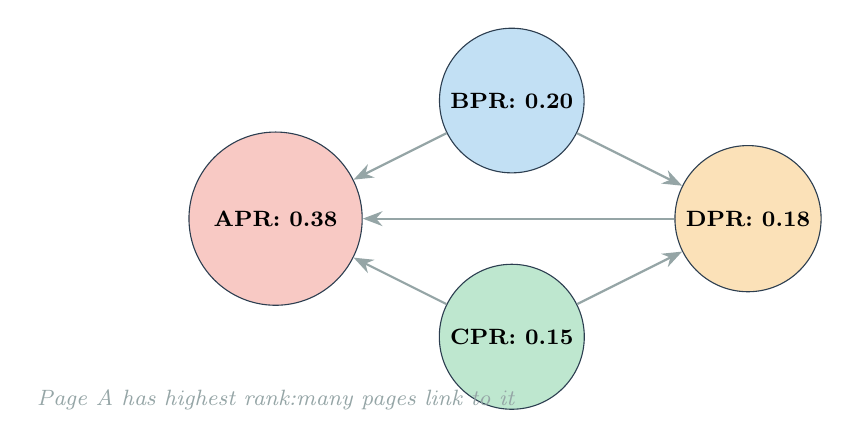
\begin{tikzpicture}[
    page/.style={circle, draw=csprimary, fill=#1, minimum size=14mm, font=\footnotesize\bfseries},
    arrow/.style={-{Stealth[length=2.5mm]}, thick, color=codegray}
]

% Pages with different PageRanks (size indicates rank)
\node[page=cssecondary!30, minimum size=22mm] (a) at (0,0) {A\newline PR: 0.38};
\node[page=cstertiary!30, minimum size=16mm] (b) at (3,1.5) {B\newline PR: 0.20};
\node[page=csaccent!30, minimum size=12mm] (c) at (3,-1.5) {C\newline PR: 0.15};
\node[page=cswarm!30, minimum size=14mm] (d) at (6,0) {D\newline PR: 0.18};

% Links
\draw[arrow] (b) -- (a);
\draw[arrow] (c) -- (a);
\draw[arrow] (d) -- (a);
\draw[arrow] (b) -- (d);
\draw[arrow] (c) -- (d);

% Annotation
\node[font=\footnotesize\itshape, color=codegray, align=center] at (0,-2.3) {Page A has highest rank:\newline many pages link to it};

\end{tikzpicture}
\end{center}

PageRank is computed iteratively: start with equal scores, then repeatedly update each page's score based on who links to it. After many iterations, the scores converge to stable values.

\begin{javacode}[Simplified PageRank Iteration]
public void computePageRank(int iterations) {
    int n = pages.size();
    double d = 0.85;  // damping factor
    
    // Initialize all pages with equal rank
    for (Page page : pages) {
        page.rank = 1.0 / n;
    }
    
    // Iterate to convergence
    for (int i = 0; i < iterations; i++) {
        for (Page page : pages) {
            double sum = 0.0;
            
            // Sum contributions from pages linking to this one
            for (Page linker : page.getIncomingLinks()) {
                sum += linker.rank / linker.getOutgoingLinkCount();
            }
            
            page.newRank = (1 - d) / n + d * sum;
        }
        
        // Update all ranks simultaneously
        for (Page page : pages) {
            page.rank = page.newRank;
        }
    }
}
\end{javacode}

Today, Google uses hundreds of ranking signals beyond PageRank---including page load speed, mobile-friendliness, content freshness, and user engagement---but PageRank remains a foundational concept.

%---------- DISTRIBUTED PROCESSING ----------%
\section{Step 4: Distributed Processing}

Even with an efficient index, no single computer could handle Google's scale. The solution: \keyterm{distributed computing}---splitting work across thousands of machines working in parallel.

\begin{historybox}[MapReduce and the Google File System]
In 2003--2004, Google published papers describing two internal systems: the Google File System (GFS) and MapReduce. These revealed how Google processed data at unprecedented scale.

GFS splits files into chunks distributed across thousands of servers, with automatic replication for reliability. MapReduce provides a programming model for parallel computation: ``map'' functions process chunks independently, then ``reduce'' functions combine results.

These papers inspired Hadoop, an open-source implementation that brought big data processing to the masses. The core insight: instead of moving data to computation, move computation to data. When your data is spread across thousands of machines, send your program to each machine rather than gathering data to one place.
\end{historybox}

When you search Google, your query doesn't go to one server---it goes to potentially thousands, each responsible for a portion of the index:

\begin{center}
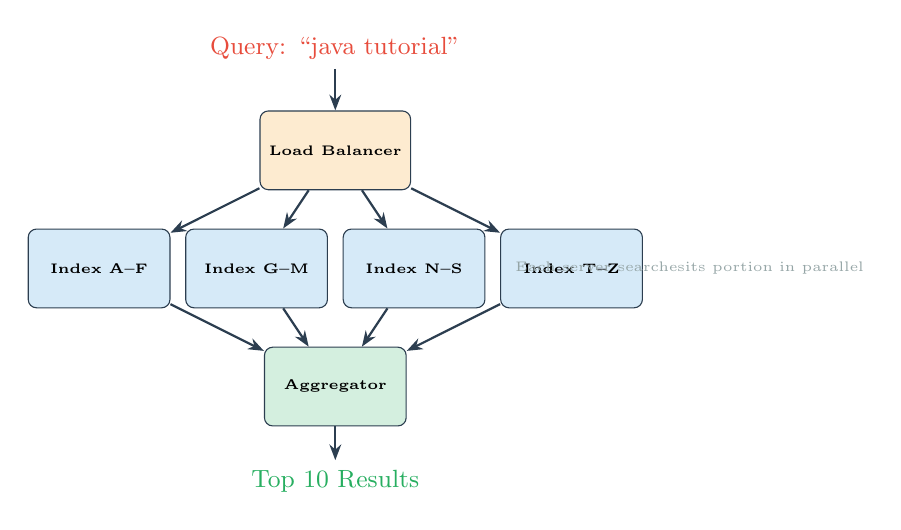
\begin{tikzpicture}[
    server/.style={rectangle, rounded corners=3pt, draw=csprimary, fill=#1, minimum width=18mm, minimum height=10mm, font=\tiny\bfseries},
    arrow/.style={-{Stealth[length=2mm]}, thick, color=csprimary}
]

% User query
\node[font=\small, color=cssecondary] (query) at (0,0) {Query: ``java tutorial''};

% Load balancer
\node[server=cswarm!20] (lb) at (0,-1.3) {Load Balancer};

% Index servers
\node[server=cstertiary!20] (s1) at (-3,-2.8) {Index A--F};
\node[server=cstertiary!20] (s2) at (-1,-2.8) {Index G--M};
\node[server=cstertiary!20] (s3) at (1,-2.8) {Index N--S};
\node[server=cstertiary!20] (s4) at (3,-2.8) {Index T--Z};

% Aggregator
\node[server=csaccent!20] (agg) at (0,-4.3) {Aggregator};

% Results
\node[font=\small, color=csaccent] (results) at (0,-5.5) {Top 10 Results};

% Arrows
\draw[arrow] (query) -- (lb);
\draw[arrow] (lb) -- (s1);
\draw[arrow] (lb) -- (s2);
\draw[arrow] (lb) -- (s3);
\draw[arrow] (lb) -- (s4);
\draw[arrow] (s1) -- (agg);
\draw[arrow] (s2) -- (agg);
\draw[arrow] (s3) -- (agg);
\draw[arrow] (s4) -- (agg);
\draw[arrow] (agg) -- (results);

% Timing
\node[font=\tiny, color=codegray] at (4.5,-2.8) {Each server searches\newline its portion in parallel};

\end{tikzpicture}
\end{center}

Each index server searches its portion simultaneously. An aggregator combines partial results, sorts by relevance, and returns the top matches. Because the work happens in parallel, adding more servers allows handling more queries, larger indexes, and faster responses.

Google's data centers contain millions of servers. Individual machines fail constantly---but the system is designed so that failures don't matter. Data is replicated across multiple servers and multiple geographic locations. If one server dies, others have copies.

%---------- QUERY PROCESSING ----------%
\section{What Happens When You Search}

Let's trace a complete search, from keystroke to results:

\begin{enumerate}[itemsep=3pt]
    \item \textbf{Query sent}: Your browser sends ``java tutorial'' to Google's servers (encrypted via HTTPS).
    
    \item \textbf{Query understanding}: Google analyzes your query. Does ``java'' mean the programming language or the island? Context clues and your search history help disambiguate. Spelling is checked; synonyms are considered.
    
    \item \textbf{Index lookup}: The query is broadcast to index servers. Each looks up ``java'' and ``tutorial'' in its portion of the inverted index, finding documents containing both words.
    
    \item \textbf{Scoring}: Matching documents are scored using hundreds of signals: PageRank, keyword prominence, freshness, mobile-friendliness, site authority, and more.
    
    \item \textbf{Aggregation}: Partial results from all servers are merged, sorted by score, and deduplicated.
    
    \item \textbf{Result generation}: For top results, Google fetches snippets (the preview text), generates any special features (videos, ``People also ask''), and assembles the response.
    
    \item \textbf{Response sent}: The complete results page is sent to your browser.
\end{enumerate}

All of this happens in under 500 milliseconds. Google reports the actual time (``About 1,350,000,000 results (0.42 seconds)'') as a point of pride---and accountability.

%---------- THE LLM REVOLUTION ----------%
\section{The LLM Revolution in Search}

For 25 years, search engines returned \textit{links}---pointers to pages where you might find answers. You still had to click, read, and synthesize information yourself. \keyterm{Large Language Models} (LLMs) are fundamentally changing this paradigm.

\begin{historybox}[ChatGPT and the Search Disruption (2022--Present)]
When OpenAI released ChatGPT in November 2022, it sent shockwaves through the tech industry. Here was a system that could directly \textit{answer} questions rather than pointing to documents. Microsoft quickly integrated similar technology into Bing (``Bing Chat,'' later ``Copilot''). Google responded with ``Bard'' (later ``Gemini'') and began adding ``AI Overviews'' directly to search results.

For the first time since Google's dominance began, the fundamental model of search---find documents, return links---faced a credible alternative: understand the question, synthesize information, generate an answer.
\end{historybox}

\subsection{How LLMs Change Search}

Traditional search is \keyterm{retrieval}: find existing documents that match your query. LLM-based search adds \keyterm{generation}: create new text that synthesizes information.

\begin{center}
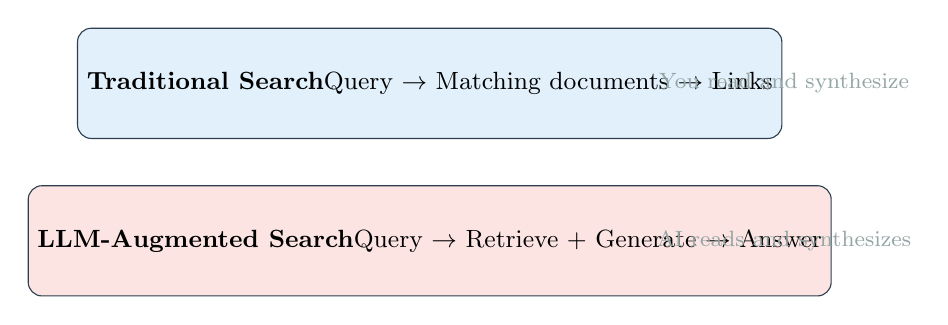
\begin{tikzpicture}[
    box/.style={rectangle, rounded corners=5pt, draw=csprimary, fill=#1, minimum width=50mm, minimum height=14mm, font=\small, align=center},
    arrow/.style={-{Stealth[length=2.5mm]}, thick, color=csprimary}
]

% Traditional search
\node[box=cstertiary!15] (trad) at (0,1) {\textbf{Traditional Search}\newline Query $\rightarrow$ Matching documents $\rightarrow$ Links};

% LLM search
\node[box=cssecondary!15] (llm) at (0,-1) {\textbf{LLM-Augmented Search}\newline Query $\rightarrow$ Retrieve + Generate $\rightarrow$ Answer};

% Annotations
\node[font=\footnotesize, color=codegray] at (4.5,1) {You read and synthesize};
\node[font=\footnotesize, color=codegray] at (4.5,-1) {AI reads and synthesizes};

\end{tikzpicture}
\end{center}

Modern systems often combine both approaches in a technique called \keyterm{Retrieval-Augmented Generation} (RAG):
\begin{enumerate}[itemsep=2pt]
    \item Use traditional search to find relevant documents
    \item Feed those documents to an LLM as context
    \item Have the LLM generate an answer based on the retrieved information
\end{enumerate}

This grounds the LLM's response in actual sources, reducing (but not eliminating) the risk of \keyterm{hallucinations}---plausible-sounding but incorrect information that LLMs sometimes generate.

\subsection{New Challenges}

LLM search introduces new problems:

\textbf{Accuracy and hallucinations.} LLMs can confidently state false information. When Google's AI Overview told users to add glue to pizza sauce (citing a satirical Reddit post), it highlighted the risks of automated answer generation.

\textbf{Source attribution.} When an LLM synthesizes an answer from multiple sources, who gets credit? How do content creators get traffic if users never click through?

\textbf{Bias and manipulation.} LLMs can perpetuate biases in their training data. They might also be manipulated by adversarial content designed to influence generated answers.

\textbf{Computational cost.} Generating text with an LLM requires far more computation than traditional search. Scaling this to billions of queries is expensive and energy-intensive.

\subsection{The Future of Search}

Search is evolving from ``finding documents'' to ``answering questions.'' The next generation may feel more like a conversation than a keyword lookup. But the fundamentals we've explored---crawling, indexing, ranking, distributed processing---remain essential. LLMs don't replace the index; they add a layer on top of it.

The question is no longer just ``which pages match your query?'' but ``what do you actually want to know, and how can we best help you learn it?'' That's a much harder problem---and an exciting frontier for computer science.

%---------- DISCUSSION QUESTIONS ----------%
\section*{Discussion Questions}

\begin{questionbox}
\begin{enumerate}[leftmargin=*, label=\textcolor{cswarm}{\textbf{\arabic*.}}]
    \item \textbf{The Power of PageRank:} PageRank treats links as votes, but not all votes are equal---links from important pages count more. What are the strengths and weaknesses of this approach? Can it be manipulated? How might it affect which voices get heard online?

    \item \textbf{Filter Bubbles:} Google personalizes results based on your search history and behavior. You might see different results than someone else searching the same query. What are the benefits and dangers of personalization? How might it affect political discourse or access to diverse viewpoints?

    \item \textbf{Search Monopoly:} Google handles over 90\% of web searches worldwide. What are the implications of one company controlling how most humans find information? Should search engines be regulated like utilities? What would meaningful competition look like?

    \item \textbf{The Content Creator's Dilemma:} If AI can summarize a web page so users don't need to visit it, what happens to the websites that created that content? How should content creators be compensated in an age of AI-generated answers? Is this fundamentally different from Google showing snippets?

    \item \textbf{Trust and Verification:} Traditional search returns sources you can evaluate. LLM-generated answers often feel authoritative even when wrong. How should AI-generated content be presented? What responsibility do users have to verify AI-provided information? What responsibility do the AI companies have?
\end{enumerate}
\end{questionbox}

%---------- GLOSSARY ----------%
\section*{Key Terms}

\begin{glossarybox}
\begin{description}[leftmargin=!, labelwidth=3.4cm, font=\bfseries\color{cssecondary}]
    \item[Crawler] A program that systematically browses the web, following links to discover and download pages for indexing.
    
    \item[Distributed Computing] Splitting computation across many machines working in parallel, enabling processing at scales impossible for single computers.
    
    \item[Hallucination] When an LLM generates plausible-sounding but factually incorrect information.
    
    \item[Index] A data structure optimized for fast lookups, mapping search terms to the documents containing them.
    
    \item[Inverted Index] An index structure mapping each word to the list of documents containing it---the foundation of web search.
    
    \item[Large Language Model] An AI system trained on vast text data that can generate human-like text and answer questions.
    
    \item[MapReduce] A programming model for processing large datasets in parallel across distributed systems.
    
    \item[PageRank] Google's original algorithm for ranking pages based on link structure, treating links as votes weighted by the linker's importance.
    
    \item[Query] The search terms a user enters, which the search engine interprets and matches against its index.
    
    \item[Ranking] Ordering search results by relevance using signals like PageRank, content quality, and user intent.
    
    \item[Retrieval-Augmented Generation] A technique combining traditional search (retrieval) with LLM text generation to ground answers in sources.
    
    \item[Web Crawler] See Crawler.
\end{description}
\end{glossarybox}

\vspace{5mm}

%---------- FOOTER ----------%
\begin{center}
\textcolor{csprimary}{\rule{0.6\textwidth}{0.5pt}}\\[3mm]
{\small\textcolor{gray}{This case study is part of the Open Educational Resources for \cscourse.\\
Licensed under Creative Commons Attribution 4.0 (CC BY 4.0).}}
\end{center}

\end{document}